\chapter{The Joints Problem \label{chap:joints}}
\begin{definition}
    Let $\LL$ be a set of distinct lines in $\RR^n$. A \textbf{joint} of $\LL$ is a point which lies in three non-coplanar lines of $\LL$.
\end{definition}
The joints problem consists in obtaining a sharp upper bound on the maximal number of joints that can be formed from a configuration of $L$ distinct lines.
We denote this quantity $J(L)$. In other words $J(L)$ is the supremum over all configurations of lines in $\RR^n$ of the number of joints.

The joints problem was first posed in 1990 by Chazelle et al in \cite{chazelle1990counting}. They focused on the 3-dimensional case of the problem, establishing a lower bound of $\Omega (N^{3/2})$ and an upper bound estimate of $O(N^{7/4})$. 
This upper bound exponent has fallen gradually throughout the years, the best result prior to the application of the polynomial method being due to Sharir and Feldman who established an upper bound of $O(N^{112/69})$. Their
proof uses an array of tools from combinatorial geometry, including forbidden subgraphs in extremal graph theory, space decomposition techniques, and some results from the geometry of lines in space.

\section{Examples}
We shall begin by examining an example based on a grid, in order to gain better intuition about the problem and formulating a conjecture. 
\begin{example}Consider an $N \times N \times N$ regular grid of integer coordinates in $\RR^3$. We shall give a collection of lines such that each point of this grid is a joint for the collection.
Let $\LL$ be the collection of all lines parallel to any of the Cartesian axes that intersect a point in this grid.
For each horizontal $N \times N$ layer, there are $N+N = 2N$ such lines that intersect our grid. 
There are $N$ layers, so we obtain $2N^2$ distinct lines in this manner. Finally we need to account for the $N^2$ lines perpendicular to the horizontal $N\times N$ layers.
This leaves us with $|\LL| = 3 N^2$ lines forming $N^3$ joints. The number of joints is thus $\sim$ $|\LL|^{3/2}$. 
\end{example}
\begin{figure}[h]
    \centering
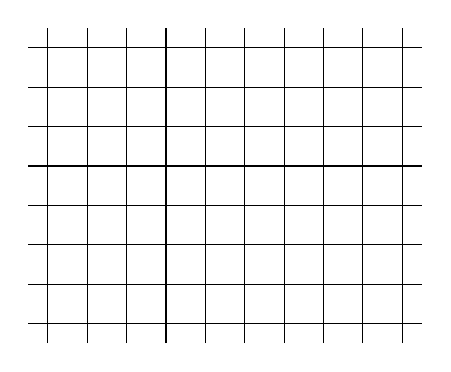
\begin{tikzpicture}
    \draw [step=0.5] (0.25,0.25) grid (5.25,4.25);
\end{tikzpicture}
\caption{A $N \times N$ layer of our grid.}
\end{figure}

We can extend this example to higher dimensional grids easily. 
\begin{example}
If we have an $\underbrace{N \times \dots \times N}_{n \text{ Dimensions}}$ regular grid of integer coordinates in $\RR^n$, we can construct an example  by a straightforward extension
of the above example. Each additional dimension increases the number of lines by a factor of $N$ (this can be seen by considering each new dimension as a layering of the previous set along the new axis).
Thus we can see that $\sim N^{n-1}$ lines form $N^n$ joints in this manner. So the number of joints is $\sim |\LL|^{\frac{n}{n-1}}$.
\end{example}

It turns out that the examples illustrated above provide asymptotically maximal configurations, that is, disregarding the best constant $C$ such that $J(L) \leq CL^{\frac{n}{n-1}}$.
\section{Solution of the Joints Problem}
This solution was first produced by Guth-Katz for the three-dimensional case,\cite{guth2008algebraic} and later extended to the general case by Quilodrán,\cite{quilodran2009joints} and independently at the same time by 
Kaplan-Sharir-Shustin.\cite{kaplan2009lines} \todo{ref}


\begin{theorem}
    In $\RR^n$ we have
      $$J(L) \lesssim_n L^{\frac{n}{n-1}}.$$
\end{theorem}
We begin with the fundamental lemma to this proof. \todo{poly method strat}
\begin{lemma}
    If $\LL$ is a set of lines in $\RR^n$ that determines $J$ joints, then one of the lines contains at most $nJ^{\frac{1}{n}}$ joints.
\label{joints_bound}
\end{lemma}
\begin{proof}
Let $P$ be a non-zero polynomial that vanishes at every joint of $\LL$ and assume that the degree of $P$ is minimal. By parameter counting (Lemma \ref{lem:paramcounting}) the degree of $P$ is at most 
$nJ^{\frac{1}{n}}$. (To see this, set $D = \lfloor nJ^{\frac{1}{n}}\rfloor$ and then notice that $J < {{D+n}\choose {n}}$.)

We proceed by contradiction. Assume every line contains more than $nJ^{\frac{1}{n}}$ joints.
 Now $P$ must vanish on every line in $\LL$ as the degree of $P$ is less than the number of joints contained in the line, which are the points of intersection between the line and $Z(P)$. \todo{check this was distracted}

We now examine the gradient of $P$ at each joint in $\LL$. We will need a fact about gradients for this, which we encapsulate in the following lemma for clarity.
\begin{lemma}
    If $x$ is a joint of $\LL$, and if a smooth function $F: \RR^n \to \RR$ vanishes on the lines of $\LL$, then $\nabla F$ vanishes at $x$. 
\end{lemma}
\begin{proof}
    The joint $x$ is contained in $n$ non-coplanar lines $l_1, \dots, l_n$ with directions $v_1, v_2, \dots , v_n$ respectively. 
    Now consider the directional derivative for a particular $v_i$:
    \[
    \frac{\partial F}{\partial v_i} = \lim_{t \to 0} \frac{ \overbrace{F(x+ tv_i)}^{F \equiv 0 \text{ on a line in $\LL$}} - \overbrace{F(x)}^{F \equiv 0 \text{ on joints}}}{t} = \frac{0}{t} = 0.    
    \]
    Notice that $ \frac{\partial F}{\partial v_i} = \langle \nabla F, v_i\rangle$ so since we have this for each $v_i$, and the set of $v_i$'s form a basis of $\RR^n$ we have that $\nabla F(x) = 0$.
\end{proof}
So we see that the partial derivatives of $P$ vanish at each joint. The derivatives are polynomials of
smaller degree than $P$ and since $P$ was assumed to be a non-zero polynomial of minimal degree that
vanishes at each joint, each derivative of $P$ must be identically zero. This implies $P$ must be
constant, which is 
a contradiction.
\end{proof}
Finally we can prove the main result. 
\begin{proof}
Lemma \ref{joints_bound} tells us that if we remove a line from our collection, we are removing at most 
$n J(L) ^{\frac{1}{n}}$ joints. By repeating this process, we get the chain of inequalities

\begin{align*}
    J(L) &\leq J(L-1) + n (J(L))^{\frac{1}{n}}\\
    &\leq J(L-2) + 2\left[ n (J(L))^{\frac{1}{n}}\right]\\
    &\leq J(L-3) + 3\left[ n (J(L))^{\frac{1}{n}}\right]\\
&\vdots\\
    &\leq L \left[ n (J(L))^{\frac{1}{n}}\right].
    \intertext{Rearranging we have}
    J(L)^ {\frac{n-1}{n}} &\lesssim_n L \\
    J(L) \lesssim_n L ^{\frac{n}{n-1}}.
\end{align*}
\end{proof}
\todo{one less line in above proof?}
